\documentclass[a4paper,uplatex]{jsarticle}


% 数式
\usepackage{amsmath,amsfonts}
\usepackage{bm}
% 画像
\usepackage[dvipdfmx]{graphicx}
\usepackage{tikz}
\usepackage{gnuplot-lua-tikz}
% フォント
\usepackage[deluxe]{otf}

\usepackage{booktabs}

\numberwithin{equation}{section}
\numberwithin{figure}{section}
\numberwithin{table}{section}

\begin{document}

\title{PRML Chapter 1}
\author{}
\date{}
\maketitle

\section{例:多項式曲線フィッティング}
実数値の入力変数\(x\)を観測し、それを用いて実数値の目標変数\(t\)を予測する回帰問題を考える。ただし、ここでは関数\(\sin(2\pi x)\)にガウス分布に従う
ランダムノイズを加えて生成した人工データを用いる。

訓練集合として、\(N\)個の観測地\(x\)を並べた\(\bm{x} \equiv (x_1,\cdots,x_N)^T\)と、それぞれに対応する観測値\(t\)を並べた\(\bm{t} \equiv (t_1,\cdots,t_N)^T\)が与えられたとする。
図\ref{fig:toy data}は、\(N=10\)の場合の人工データの例である。

我々の目標は、この訓練集合を利用して、新たな入力変数\(\hat{x}\)に対して目標変数\(\hat{t}\)の値を予測することである。

\begin{figure}[htbp]
  \centering
  \begin{tikzpicture}[gnuplot]
%% generated with GNUPLOT 5.4p2 (Lua 5.4; terminal rev. Jun 2020, script rev. 114)
%% Wed Feb  7 22:18:47 2024
\path (0.000,0.000) rectangle (12.500,8.750);
\gpcolor{color=gp lt color border}
\gpsetlinetype{gp lt border}
\gpsetdashtype{gp dt solid}
\gpsetlinewidth{1.00}
\draw[gp path] (1.504,1.555)--(1.684,1.555);
\draw[gp path] (11.947,1.555)--(11.767,1.555);
\node[gp node right] at (1.320,1.555) {$-1$};
\draw[gp path] (1.504,2.980)--(1.684,2.980);
\draw[gp path] (11.947,2.980)--(11.767,2.980);
\node[gp node right] at (1.320,2.980) {$-0.5$};
\draw[gp path] (1.504,4.405)--(1.684,4.405);
\draw[gp path] (11.947,4.405)--(11.767,4.405);
\node[gp node right] at (1.320,4.405) {$0$};
\draw[gp path] (1.504,5.830)--(1.684,5.830);
\draw[gp path] (11.947,5.830)--(11.767,5.830);
\node[gp node right] at (1.320,5.830) {$0.5$};
\draw[gp path] (1.504,7.255)--(1.684,7.255);
\draw[gp path] (11.947,7.255)--(11.767,7.255);
\node[gp node right] at (1.320,7.255) {$1$};
\draw[gp path] (2.374,0.985)--(2.374,1.165);
\draw[gp path] (2.374,7.825)--(2.374,7.645);
\node[gp node center] at (2.374,0.677) {$0$};
\draw[gp path] (4.115,0.985)--(4.115,1.165);
\draw[gp path] (4.115,7.825)--(4.115,7.645);
\node[gp node center] at (4.115,0.677) {$0.2$};
\draw[gp path] (5.855,0.985)--(5.855,1.165);
\draw[gp path] (5.855,7.825)--(5.855,7.645);
\node[gp node center] at (5.855,0.677) {$0.4$};
\draw[gp path] (7.596,0.985)--(7.596,1.165);
\draw[gp path] (7.596,7.825)--(7.596,7.645);
\node[gp node center] at (7.596,0.677) {$0.6$};
\draw[gp path] (9.336,0.985)--(9.336,1.165);
\draw[gp path] (9.336,7.825)--(9.336,7.645);
\node[gp node center] at (9.336,0.677) {$0.8$};
\draw[gp path] (11.077,0.985)--(11.077,1.165);
\draw[gp path] (11.077,7.825)--(11.077,7.645);
\node[gp node center] at (11.077,0.677) {$1$};
\draw[gp path] (1.504,7.825)--(1.504,0.985)--(11.947,0.985)--(11.947,7.825)--cycle;
\node[gp node center,rotate=-270] at (0.292,4.405) {$t$};
\node[gp node center] at (6.725,0.215) {$x$};
\node[gp node right] at (10.479,7.491) {$\sin(2\pi x)$};
\gpcolor{rgb color={0.000,1.000,0.000}}
\draw[gp path] (10.663,7.491)--(11.579,7.491);
\draw[gp path] (1.504,2.730)--(1.609,2.910)--(1.715,3.099)--(1.820,3.296)--(1.926,3.499)%
  --(2.031,3.707)--(2.137,3.919)--(2.242,4.134)--(2.348,4.351)--(2.453,4.568)--(2.559,4.784)%
  --(2.664,4.998)--(2.770,5.208)--(2.875,5.414)--(2.981,5.614)--(3.086,5.806)--(3.192,5.991)%
  --(3.297,6.167)--(3.403,6.332)--(3.508,6.486)--(3.614,6.628)--(3.719,6.758)--(3.825,6.873)%
  --(3.930,6.974)--(4.036,7.061)--(4.141,7.132)--(4.247,7.187)--(4.352,7.226)--(4.458,7.249)%
  --(4.563,7.255)--(4.669,7.245)--(4.774,7.218)--(4.880,7.175)--(4.985,7.116)--(5.090,7.041)%
  --(5.196,6.950)--(5.301,6.846)--(5.407,6.727)--(5.512,6.594)--(5.618,6.449)--(5.723,6.292)%
  --(5.829,6.124)--(5.934,5.946)--(6.040,5.759)--(6.145,5.564)--(6.251,5.363)--(6.356,5.156)%
  --(6.462,4.944)--(6.567,4.730)--(6.673,4.514)--(6.778,4.296)--(6.884,4.080)--(6.989,3.866)%
  --(7.095,3.654)--(7.200,3.447)--(7.306,3.246)--(7.411,3.051)--(7.517,2.864)--(7.622,2.686)%
  --(7.728,2.518)--(7.833,2.361)--(7.939,2.216)--(8.044,2.083)--(8.150,1.964)--(8.255,1.860)%
  --(8.361,1.769)--(8.466,1.694)--(8.571,1.635)--(8.677,1.592)--(8.782,1.565)--(8.888,1.555)%
  --(8.993,1.561)--(9.099,1.584)--(9.204,1.623)--(9.310,1.678)--(9.415,1.749)--(9.521,1.836)%
  --(9.626,1.937)--(9.732,2.052)--(9.837,2.182)--(9.943,2.324)--(10.048,2.478)--(10.154,2.643)%
  --(10.259,2.819)--(10.365,3.004)--(10.470,3.196)--(10.576,3.396)--(10.681,3.602)--(10.787,3.812)%
  --(10.892,4.026)--(10.998,4.242)--(11.103,4.459)--(11.209,4.676)--(11.314,4.891)--(11.420,5.103)%
  --(11.525,5.311)--(11.631,5.514)--(11.736,5.711)--(11.842,5.900)--(11.947,6.080);
\gpcolor{color=gp lt color border}
\node[gp node right] at (10.479,7.183) {$\sin(2\pi x) + noise$};
\gpcolor{rgb color={0.000,0.000,1.000}}
\gpsetpointsize{4.00}
\gp3point{gp mark 7}{}{(2.374,4.091)}
\gp3point{gp mark 7}{}{(3.332,6.457)}
\gp3point{gp mark 7}{}{(4.289,7.056)}
\gp3point{gp mark 7}{}{(5.246,6.229)}
\gp3point{gp mark 7}{}{(6.203,5.004)}
\gp3point{gp mark 7}{}{(7.248,3.294)}
\gp3point{gp mark 7}{}{(8.205,1.355)}
\gp3point{gp mark 7}{}{(9.162,1.099)}
\gp3point{gp mark 7}{}{(10.119,3.208)}
\gp3point{gp mark 7}{}{(11.077,4.890)}
\gp3point{gp mark 7}{}{(11.121,7.183)}
\gpcolor{color=gp lt color border}
\draw[gp path] (1.504,7.825)--(1.504,0.985)--(11.947,0.985)--(11.947,7.825)--cycle;
\node[gp node center] at (6.725,8.287) {Toy Dataset};
%% coordinates of the plot area
\gpdefrectangularnode{gp plot 1}{\pgfpoint{1.504cm}{0.985cm}}{\pgfpoint{11.947cm}{7.825cm}}
\end{tikzpicture}

  \caption{\(N=10\)個の訓練データの例}
  \label{fig:toy data}
\end{figure}

ここでは、以下のような多項式を用いてデータへのフィッティングを行うことにする。
\begin{equation}
  y(x,\bm{w}) = w_0 + w_1 x + w_2 x^2 + \cdots + w_M x^M = \sum_{j=0}^{M} w_j x^j
\end{equation}
ただし、\(M\)は多項式の\textbf{次数(order)}で、\(x^j\)は\(x\)の\(j\)乗を表す。多項式の係数\(w_0,\cdots,w_M\)をまとめて\(\bm{w}\)と書くことにする。
多項式\(y(x,\bm{w})\)は、\(x\)の非線形関数であるが、係数\(\bm{w}\)の線形関数であることに注意する。このような、未知パラメータに対して線形な関数は\textbf{線形モデル}と呼ばれる。

訓練データに多項式をあてはめることで係数の値を求める。これは、\(\bm{w}\)を任意に固定したときの関数\(y(x,\bm{w})\)と
訓練集合のデータ点との間のずれを測る\textbf{誤差関数(error function)}の最小化で達成できる。ここでは、誤差関数として単純で広く用いられている\textbf{二乗和誤差(sum-of-squares error)}を用いる。
式で書けば、
\begin{equation}
  E(\bm{w}) = \frac{1}{2} \sum_{n=1}^{N} \{y(x_n,\bm{w}) - t_n\}^2
  \label{eq:sum of squares error}
\end{equation}
となる。ただし、後で便利なように係数\(1/2\)をかけている。

このように、\(E(\bm{w})\)をできるだけ小さくするような\(\bm{w}\)を選ぶことで曲線当てはめ問題を解くことができる。では、誤差関数を最小にする解\(\bm{w^*}=\{w_i\}\)を求める。
誤差関数を最小にする解をもとめるには、\(E(\bm{w})\)を\(w_i\)について微分し、その微分がゼロになるような\(w_i\)を求めればよい。
つまり、
\begin{equation}
  \frac{\delta E}{\delta w_i} = 0
\end{equation}
を求める。
はじめに、\(E(\bm{w})\)を\(w_i\)について微分する。
\begin{align*}
  \frac{\delta E}{\delta w_i} &= \frac{1}{2}\sum_{n=1}^{N}\left\{2\left(\sum_{j=0}^{M}w_j x_n^j-t_n\right)-x_n^i\right\} \\
                              &= \sum_{n=1}^{N}\left(x_n^i\sum_{j=0}^{M}w_j x_n^j\right) - \sum_{n=1}^{N}t_n x_n^i \\
\end{align*}
ここで、\(\frac{\delta E}{\delta w_i} = 0\)を求めるので、
\begin{equation}
  \sum_{n=1}^{N}\left(x_n^i\sum_{j=0}^{M}w_j x_n^j\right) = \sum_{n=1}^{N}t_n x_n^i
\end{equation}

左辺を変形すると、
\begin{align*}
  (左辺) &= \sum_{n=1}^{N}\left\{x_n^i\left(w_0 x_n^0+w_1x_n^1+\cdots+w_Mx_n^M\right)\right\} \\
         &= \sum_{n=1}^{N}\left\{w_0x_n^{i+0}+w_1x_n^{i+1}+\cdots+w_Mx_n^{i+M}\right\} \\
         &= \sum_{n=1}^{N}\sum_{j=0}^{M}\left(w_jx_n^{i+j}\right) \\
         &= \sum_{j=0}^{M}\left\{\sum_{n=1}^{N}(x_n)^{i+j}\right\}w_j \\
\end{align*}
また、
\begin{equation}
  A_{ij} = \sum_{n=1}^{N}(x_n)^{i+j}, T_i = \sum_{n=1}^{N}t_n(x_n)^i
\end{equation}
とおくと、
\begin{equation}
  \sum_{j=0}^{M}A_{ij}w_j = T_i
\end{equation}
となる。これは線形方程式であり、これを解くことで、誤差関数を最小にする解\(\bm{w^*}\)を求めることができる。

多項式の次数\(M\)を選ぶのは、\textbf{モデル比較(model comparison)}あるいは\textbf{モデル選択(model selection)}と呼ばれる問題である。例として
図\ref{fig:various M}に、\(M=0,1,3,9\)の場合のフィッティング結果を示す。

\begin{figure}[htbp]
  \centering
  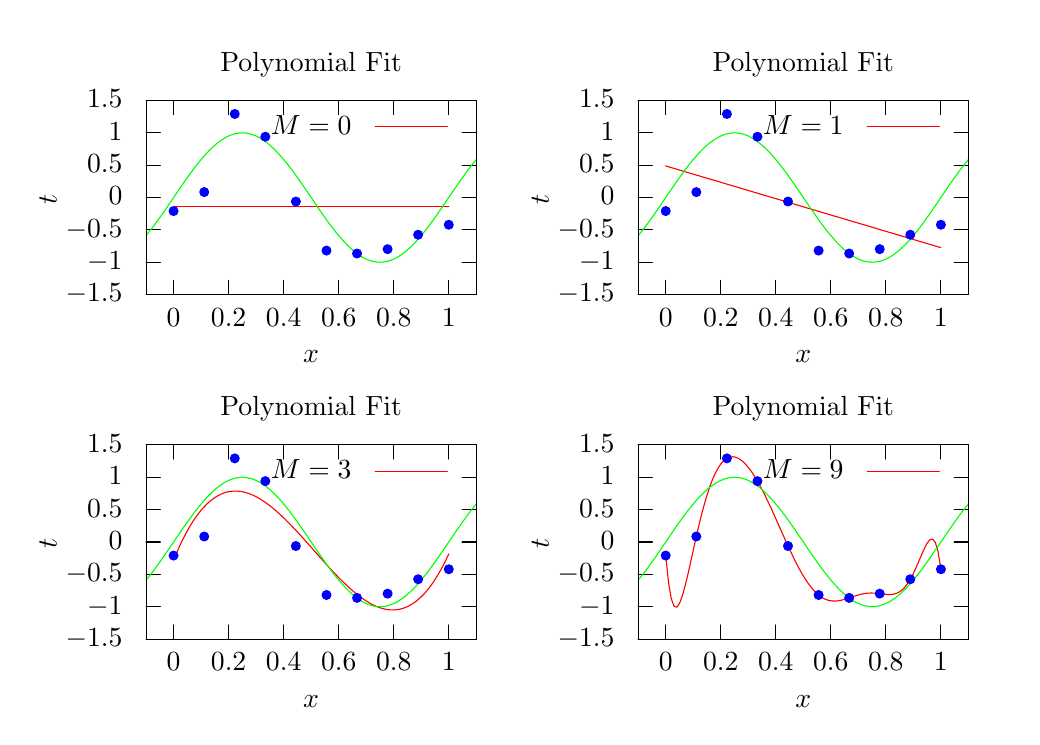
\begin{tikzpicture}[gnuplot]
%% generated with GNUPLOT 5.4p2 (Lua 5.4; terminal rev. Jun 2020, script rev. 114)
%% Fri Feb  9 11:16:22 2024
\path (0.000,0.000) rectangle (12.500,8.750);
\gpcolor{color=gp lt color border}
\gpsetlinetype{gp lt border}
\gpsetdashtype{gp dt solid}
\gpsetlinewidth{1.00}
\draw[gp path] (1.504,5.360)--(1.684,5.360);
\draw[gp path] (5.697,5.360)--(5.517,5.360);
\node[gp node right] at (1.320,5.360) {$-1.5$};
\draw[gp path] (1.504,5.771)--(1.684,5.771);
\draw[gp path] (5.697,5.771)--(5.517,5.771);
\node[gp node right] at (1.320,5.771) {$-1$};
\draw[gp path] (1.504,6.182)--(1.684,6.182);
\draw[gp path] (5.697,6.182)--(5.517,6.182);
\node[gp node right] at (1.320,6.182) {$-0.5$};
\draw[gp path] (1.504,6.593)--(1.684,6.593);
\draw[gp path] (5.697,6.593)--(5.517,6.593);
\node[gp node right] at (1.320,6.593) {$0$};
\draw[gp path] (1.504,7.003)--(1.684,7.003);
\draw[gp path] (5.697,7.003)--(5.517,7.003);
\node[gp node right] at (1.320,7.003) {$0.5$};
\draw[gp path] (1.504,7.414)--(1.684,7.414);
\draw[gp path] (5.697,7.414)--(5.517,7.414);
\node[gp node right] at (1.320,7.414) {$1$};
\draw[gp path] (1.504,7.825)--(1.684,7.825);
\draw[gp path] (5.697,7.825)--(5.517,7.825);
\node[gp node right] at (1.320,7.825) {$1.5$};
\draw[gp path] (1.853,5.360)--(1.853,5.540);
\draw[gp path] (1.853,7.825)--(1.853,7.645);
\node[gp node center] at (1.853,5.052) {$0$};
\draw[gp path] (2.552,5.360)--(2.552,5.540);
\draw[gp path] (2.552,7.825)--(2.552,7.645);
\node[gp node center] at (2.552,5.052) {$0.2$};
\draw[gp path] (3.251,5.360)--(3.251,5.540);
\draw[gp path] (3.251,7.825)--(3.251,7.645);
\node[gp node center] at (3.251,5.052) {$0.4$};
\draw[gp path] (3.950,5.360)--(3.950,5.540);
\draw[gp path] (3.950,7.825)--(3.950,7.645);
\node[gp node center] at (3.950,5.052) {$0.6$};
\draw[gp path] (4.649,5.360)--(4.649,5.540);
\draw[gp path] (4.649,7.825)--(4.649,7.645);
\node[gp node center] at (4.649,5.052) {$0.8$};
\draw[gp path] (5.348,5.360)--(5.348,5.540);
\draw[gp path] (5.348,7.825)--(5.348,7.645);
\node[gp node center] at (5.348,5.052) {$1$};
\draw[gp path] (1.504,7.825)--(1.504,5.360)--(5.697,5.360)--(5.697,7.825)--cycle;
\node[gp node center,rotate=-270] at (0.292,6.592) {$t$};
\node[gp node center] at (3.600,4.590) {$x$};
\node[gp node right] at (4.229,7.491) {$M=0$};
\gpcolor{rgb color={1.000,0.000,0.000}}
\draw[gp path] (4.413,7.491)--(5.329,7.491);
\draw[gp path] (1.853,6.475)--(1.889,6.475)--(1.924,6.475)--(1.959,6.475)--(1.995,6.475)%
  --(2.030,6.475)--(2.065,6.475)--(2.100,6.475)--(2.136,6.475)--(2.171,6.475)--(2.206,6.475)%
  --(2.242,6.475)--(2.277,6.475)--(2.312,6.475)--(2.348,6.475)--(2.383,6.475)--(2.418,6.475)%
  --(2.453,6.475)--(2.489,6.475)--(2.524,6.475)--(2.559,6.475)--(2.595,6.475)--(2.630,6.475)%
  --(2.665,6.475)--(2.700,6.475)--(2.736,6.475)--(2.771,6.475)--(2.806,6.475)--(2.842,6.475)%
  --(2.877,6.475)--(2.912,6.475)--(2.948,6.475)--(2.983,6.475)--(3.018,6.475)--(3.053,6.475)%
  --(3.089,6.475)--(3.124,6.475)--(3.159,6.475)--(3.195,6.475)--(3.230,6.475)--(3.265,6.475)%
  --(3.300,6.475)--(3.336,6.475)--(3.371,6.475)--(3.406,6.475)--(3.442,6.475)--(3.477,6.475)%
  --(3.512,6.475)--(3.548,6.475)--(3.583,6.475)--(3.618,6.475)--(3.653,6.475)--(3.689,6.475)%
  --(3.724,6.475)--(3.759,6.475)--(3.795,6.475)--(3.830,6.475)--(3.865,6.475)--(3.901,6.475)%
  --(3.936,6.475)--(3.971,6.475)--(4.006,6.475)--(4.042,6.475)--(4.077,6.475)--(4.112,6.475)%
  --(4.148,6.475)--(4.183,6.475)--(4.218,6.475)--(4.253,6.475)--(4.289,6.475)--(4.324,6.475)%
  --(4.359,6.475)--(4.395,6.475)--(4.430,6.475)--(4.465,6.475)--(4.501,6.475)--(4.536,6.475)%
  --(4.571,6.475)--(4.606,6.475)--(4.642,6.475)--(4.677,6.475)--(4.712,6.475)--(4.748,6.475)%
  --(4.783,6.475)--(4.818,6.475)--(4.853,6.475)--(4.889,6.475)--(4.924,6.475)--(4.959,6.475)%
  --(4.995,6.475)--(5.030,6.475)--(5.065,6.475)--(5.101,6.475)--(5.136,6.475)--(5.171,6.475)%
  --(5.206,6.475)--(5.242,6.475)--(5.277,6.475)--(5.312,6.475)--(5.348,6.475);
\gpcolor{rgb color={0.000,1.000,0.000}}
\draw[gp path] (1.504,6.110)--(1.546,6.162)--(1.589,6.216)--(1.631,6.273)--(1.673,6.331)%
  --(1.716,6.391)--(1.758,6.452)--(1.800,6.514)--(1.843,6.577)--(1.885,6.639)--(1.928,6.702)%
  --(1.970,6.763)--(2.012,6.824)--(2.055,6.883)--(2.097,6.941)--(2.139,6.997)--(2.182,7.050)%
  --(2.224,7.100)--(2.266,7.148)--(2.309,7.193)--(2.351,7.234)--(2.393,7.271)--(2.436,7.304)%
  --(2.478,7.333)--(2.520,7.358)--(2.563,7.379)--(2.605,7.395)--(2.648,7.406)--(2.690,7.412)%
  --(2.732,7.414)--(2.775,7.411)--(2.817,7.403)--(2.859,7.391)--(2.902,7.374)--(2.944,7.352)%
  --(2.986,7.326)--(3.029,7.296)--(3.071,7.262)--(3.113,7.224)--(3.156,7.182)--(3.198,7.136)%
  --(3.240,7.088)--(3.283,7.037)--(3.325,6.983)--(3.368,6.927)--(3.410,6.869)--(3.452,6.809)%
  --(3.495,6.748)--(3.537,6.686)--(3.579,6.624)--(3.622,6.561)--(3.664,6.499)--(3.706,6.437)%
  --(3.749,6.376)--(3.791,6.316)--(3.833,6.258)--(3.876,6.202)--(3.918,6.148)--(3.961,6.097)%
  --(4.003,6.049)--(4.045,6.003)--(4.088,5.961)--(4.130,5.923)--(4.172,5.889)--(4.215,5.859)%
  --(4.257,5.833)--(4.299,5.811)--(4.342,5.794)--(4.384,5.782)--(4.426,5.774)--(4.469,5.771)%
  --(4.511,5.773)--(4.553,5.779)--(4.596,5.790)--(4.638,5.806)--(4.681,5.827)--(4.723,5.852)%
  --(4.765,5.881)--(4.808,5.914)--(4.850,5.951)--(4.892,5.992)--(4.935,6.037)--(4.977,6.085)%
  --(5.019,6.135)--(5.062,6.188)--(5.104,6.244)--(5.146,6.302)--(5.189,6.361)--(5.231,6.422)%
  --(5.273,6.483)--(5.316,6.546)--(5.358,6.608)--(5.401,6.671)--(5.443,6.733)--(5.485,6.794)%
  --(5.528,6.854)--(5.570,6.912)--(5.612,6.969)--(5.655,7.023)--(5.697,7.075);
\gpcolor{rgb color={0.000,0.000,1.000}}
\gpsetpointsize{4.00}
\gp3point{gp mark 7}{}{(1.853,6.421)}
\gp3point{gp mark 7}{}{(2.242,6.662)}
\gp3point{gp mark 7}{}{(2.630,7.654)}
\gp3point{gp mark 7}{}{(3.018,7.365)}
\gp3point{gp mark 7}{}{(3.406,6.542)}
\gp3point{gp mark 7}{}{(3.795,5.919)}
\gp3point{gp mark 7}{}{(4.183,5.882)}
\gp3point{gp mark 7}{}{(4.571,5.937)}
\gp3point{gp mark 7}{}{(4.959,6.120)}
\gp3point{gp mark 7}{}{(5.348,6.247)}
\gpcolor{color=gp lt color border}
\draw[gp path] (1.504,7.825)--(1.504,5.360)--(5.697,5.360)--(5.697,7.825)--cycle;
\node[gp node center] at (3.600,8.287) {Polynomial Fit};
%% coordinates of the plot area
\gpdefrectangularnode{gp plot 1}{\pgfpoint{1.504cm}{5.360cm}}{\pgfpoint{5.697cm}{7.825cm}}
\draw[gp path] (7.754,5.360)--(7.934,5.360);
\draw[gp path] (11.947,5.360)--(11.767,5.360);
\node[gp node right] at (7.570,5.360) {$-1.5$};
\draw[gp path] (7.754,5.771)--(7.934,5.771);
\draw[gp path] (11.947,5.771)--(11.767,5.771);
\node[gp node right] at (7.570,5.771) {$-1$};
\draw[gp path] (7.754,6.182)--(7.934,6.182);
\draw[gp path] (11.947,6.182)--(11.767,6.182);
\node[gp node right] at (7.570,6.182) {$-0.5$};
\draw[gp path] (7.754,6.593)--(7.934,6.593);
\draw[gp path] (11.947,6.593)--(11.767,6.593);
\node[gp node right] at (7.570,6.593) {$0$};
\draw[gp path] (7.754,7.003)--(7.934,7.003);
\draw[gp path] (11.947,7.003)--(11.767,7.003);
\node[gp node right] at (7.570,7.003) {$0.5$};
\draw[gp path] (7.754,7.414)--(7.934,7.414);
\draw[gp path] (11.947,7.414)--(11.767,7.414);
\node[gp node right] at (7.570,7.414) {$1$};
\draw[gp path] (7.754,7.825)--(7.934,7.825);
\draw[gp path] (11.947,7.825)--(11.767,7.825);
\node[gp node right] at (7.570,7.825) {$1.5$};
\draw[gp path] (8.103,5.360)--(8.103,5.540);
\draw[gp path] (8.103,7.825)--(8.103,7.645);
\node[gp node center] at (8.103,5.052) {$0$};
\draw[gp path] (8.802,5.360)--(8.802,5.540);
\draw[gp path] (8.802,7.825)--(8.802,7.645);
\node[gp node center] at (8.802,5.052) {$0.2$};
\draw[gp path] (9.501,5.360)--(9.501,5.540);
\draw[gp path] (9.501,7.825)--(9.501,7.645);
\node[gp node center] at (9.501,5.052) {$0.4$};
\draw[gp path] (10.200,5.360)--(10.200,5.540);
\draw[gp path] (10.200,7.825)--(10.200,7.645);
\node[gp node center] at (10.200,5.052) {$0.6$};
\draw[gp path] (10.899,5.360)--(10.899,5.540);
\draw[gp path] (10.899,7.825)--(10.899,7.645);
\node[gp node center] at (10.899,5.052) {$0.8$};
\draw[gp path] (11.598,5.360)--(11.598,5.540);
\draw[gp path] (11.598,7.825)--(11.598,7.645);
\node[gp node center] at (11.598,5.052) {$1$};
\draw[gp path] (7.754,7.825)--(7.754,5.360)--(11.947,5.360)--(11.947,7.825)--cycle;
\node[gp node center,rotate=-270] at (6.542,6.592) {$t$};
\node[gp node center] at (9.850,4.590) {$x$};
\node[gp node right] at (10.479,7.491) {$M=1$};
\gpcolor{rgb color={1.000,0.000,0.000}}
\draw[gp path] (10.663,7.491)--(11.579,7.491);
\draw[gp path] (8.103,6.994)--(8.139,6.983)--(8.174,6.973)--(8.209,6.962)--(8.245,6.952)%
  --(8.280,6.941)--(8.315,6.931)--(8.350,6.920)--(8.386,6.910)--(8.421,6.899)--(8.456,6.889)%
  --(8.492,6.878)--(8.527,6.868)--(8.562,6.857)--(8.598,6.847)--(8.633,6.836)--(8.668,6.826)%
  --(8.703,6.816)--(8.739,6.805)--(8.774,6.795)--(8.809,6.784)--(8.845,6.774)--(8.880,6.763)%
  --(8.915,6.753)--(8.950,6.742)--(8.986,6.732)--(9.021,6.721)--(9.056,6.711)--(9.092,6.700)%
  --(9.127,6.690)--(9.162,6.679)--(9.198,6.669)--(9.233,6.658)--(9.268,6.648)--(9.303,6.637)%
  --(9.339,6.627)--(9.374,6.616)--(9.409,6.606)--(9.445,6.595)--(9.480,6.585)--(9.515,6.575)%
  --(9.550,6.564)--(9.586,6.554)--(9.621,6.543)--(9.656,6.533)--(9.692,6.522)--(9.727,6.512)%
  --(9.762,6.501)--(9.798,6.491)--(9.833,6.480)--(9.868,6.470)--(9.903,6.459)--(9.939,6.449)%
  --(9.974,6.438)--(10.009,6.428)--(10.045,6.417)--(10.080,6.407)--(10.115,6.396)--(10.151,6.386)%
  --(10.186,6.375)--(10.221,6.365)--(10.256,6.354)--(10.292,6.344)--(10.327,6.334)--(10.362,6.323)%
  --(10.398,6.313)--(10.433,6.302)--(10.468,6.292)--(10.503,6.281)--(10.539,6.271)--(10.574,6.260)%
  --(10.609,6.250)--(10.645,6.239)--(10.680,6.229)--(10.715,6.218)--(10.751,6.208)--(10.786,6.197)%
  --(10.821,6.187)--(10.856,6.176)--(10.892,6.166)--(10.927,6.155)--(10.962,6.145)--(10.998,6.134)%
  --(11.033,6.124)--(11.068,6.113)--(11.103,6.103)--(11.139,6.093)--(11.174,6.082)--(11.209,6.072)%
  --(11.245,6.061)--(11.280,6.051)--(11.315,6.040)--(11.351,6.030)--(11.386,6.019)--(11.421,6.009)%
  --(11.456,5.998)--(11.492,5.988)--(11.527,5.977)--(11.562,5.967)--(11.598,5.956);
\gpcolor{rgb color={0.000,1.000,0.000}}
\draw[gp path] (7.754,6.110)--(7.796,6.162)--(7.839,6.216)--(7.881,6.273)--(7.923,6.331)%
  --(7.966,6.391)--(8.008,6.452)--(8.050,6.514)--(8.093,6.577)--(8.135,6.639)--(8.178,6.702)%
  --(8.220,6.763)--(8.262,6.824)--(8.305,6.883)--(8.347,6.941)--(8.389,6.997)--(8.432,7.050)%
  --(8.474,7.100)--(8.516,7.148)--(8.559,7.193)--(8.601,7.234)--(8.643,7.271)--(8.686,7.304)%
  --(8.728,7.333)--(8.770,7.358)--(8.813,7.379)--(8.855,7.395)--(8.898,7.406)--(8.940,7.412)%
  --(8.982,7.414)--(9.025,7.411)--(9.067,7.403)--(9.109,7.391)--(9.152,7.374)--(9.194,7.352)%
  --(9.236,7.326)--(9.279,7.296)--(9.321,7.262)--(9.363,7.224)--(9.406,7.182)--(9.448,7.136)%
  --(9.490,7.088)--(9.533,7.037)--(9.575,6.983)--(9.618,6.927)--(9.660,6.869)--(9.702,6.809)%
  --(9.745,6.748)--(9.787,6.686)--(9.829,6.624)--(9.872,6.561)--(9.914,6.499)--(9.956,6.437)%
  --(9.999,6.376)--(10.041,6.316)--(10.083,6.258)--(10.126,6.202)--(10.168,6.148)--(10.211,6.097)%
  --(10.253,6.049)--(10.295,6.003)--(10.338,5.961)--(10.380,5.923)--(10.422,5.889)--(10.465,5.859)%
  --(10.507,5.833)--(10.549,5.811)--(10.592,5.794)--(10.634,5.782)--(10.676,5.774)--(10.719,5.771)%
  --(10.761,5.773)--(10.803,5.779)--(10.846,5.790)--(10.888,5.806)--(10.931,5.827)--(10.973,5.852)%
  --(11.015,5.881)--(11.058,5.914)--(11.100,5.951)--(11.142,5.992)--(11.185,6.037)--(11.227,6.085)%
  --(11.269,6.135)--(11.312,6.188)--(11.354,6.244)--(11.396,6.302)--(11.439,6.361)--(11.481,6.422)%
  --(11.523,6.483)--(11.566,6.546)--(11.608,6.608)--(11.651,6.671)--(11.693,6.733)--(11.735,6.794)%
  --(11.778,6.854)--(11.820,6.912)--(11.862,6.969)--(11.905,7.023)--(11.947,7.075);
\gpcolor{rgb color={0.000,0.000,1.000}}
\gp3point{gp mark 7}{}{(8.103,6.421)}
\gp3point{gp mark 7}{}{(8.492,6.662)}
\gp3point{gp mark 7}{}{(8.880,7.654)}
\gp3point{gp mark 7}{}{(9.268,7.365)}
\gp3point{gp mark 7}{}{(9.656,6.542)}
\gp3point{gp mark 7}{}{(10.045,5.919)}
\gp3point{gp mark 7}{}{(10.433,5.882)}
\gp3point{gp mark 7}{}{(10.821,5.937)}
\gp3point{gp mark 7}{}{(11.209,6.120)}
\gp3point{gp mark 7}{}{(11.598,6.247)}
\gpcolor{color=gp lt color border}
\draw[gp path] (7.754,7.825)--(7.754,5.360)--(11.947,5.360)--(11.947,7.825)--cycle;
\node[gp node center] at (9.850,8.287) {Polynomial Fit};
%% coordinates of the plot area
\gpdefrectangularnode{gp plot 2}{\pgfpoint{7.754cm}{5.360cm}}{\pgfpoint{11.947cm}{7.825cm}}
\draw[gp path] (1.504,0.985)--(1.684,0.985);
\draw[gp path] (5.697,0.985)--(5.517,0.985);
\node[gp node right] at (1.320,0.985) {$-1.5$};
\draw[gp path] (1.504,1.396)--(1.684,1.396);
\draw[gp path] (5.697,1.396)--(5.517,1.396);
\node[gp node right] at (1.320,1.396) {$-1$};
\draw[gp path] (1.504,1.807)--(1.684,1.807);
\draw[gp path] (5.697,1.807)--(5.517,1.807);
\node[gp node right] at (1.320,1.807) {$-0.5$};
\draw[gp path] (1.504,2.218)--(1.684,2.218);
\draw[gp path] (5.697,2.218)--(5.517,2.218);
\node[gp node right] at (1.320,2.218) {$0$};
\draw[gp path] (1.504,2.629)--(1.684,2.629);
\draw[gp path] (5.697,2.629)--(5.517,2.629);
\node[gp node right] at (1.320,2.629) {$0.5$};
\draw[gp path] (1.504,3.040)--(1.684,3.040);
\draw[gp path] (5.697,3.040)--(5.517,3.040);
\node[gp node right] at (1.320,3.040) {$1$};
\draw[gp path] (1.504,3.451)--(1.684,3.451);
\draw[gp path] (5.697,3.451)--(5.517,3.451);
\node[gp node right] at (1.320,3.451) {$1.5$};
\draw[gp path] (1.853,0.985)--(1.853,1.165);
\draw[gp path] (1.853,3.451)--(1.853,3.271);
\node[gp node center] at (1.853,0.677) {$0$};
\draw[gp path] (2.552,0.985)--(2.552,1.165);
\draw[gp path] (2.552,3.451)--(2.552,3.271);
\node[gp node center] at (2.552,0.677) {$0.2$};
\draw[gp path] (3.251,0.985)--(3.251,1.165);
\draw[gp path] (3.251,3.451)--(3.251,3.271);
\node[gp node center] at (3.251,0.677) {$0.4$};
\draw[gp path] (3.950,0.985)--(3.950,1.165);
\draw[gp path] (3.950,3.451)--(3.950,3.271);
\node[gp node center] at (3.950,0.677) {$0.6$};
\draw[gp path] (4.649,0.985)--(4.649,1.165);
\draw[gp path] (4.649,3.451)--(4.649,3.271);
\node[gp node center] at (4.649,0.677) {$0.8$};
\draw[gp path] (5.348,0.985)--(5.348,1.165);
\draw[gp path] (5.348,3.451)--(5.348,3.271);
\node[gp node center] at (5.348,0.677) {$1$};
\draw[gp path] (1.504,3.451)--(1.504,0.985)--(5.697,0.985)--(5.697,3.451)--cycle;
\node[gp node center,rotate=-270] at (0.292,2.218) {$t$};
\node[gp node center] at (3.600,0.215) {$x$};
\node[gp node right] at (4.229,3.117) {$M=3$};
\gpcolor{rgb color={1.000,0.000,0.000}}
\draw[gp path] (4.413,3.117)--(5.329,3.117);
\draw[gp path] (1.853,1.989)--(1.889,2.074)--(1.924,2.153)--(1.959,2.228)--(1.995,2.298)%
  --(2.030,2.364)--(2.065,2.425)--(2.100,2.482)--(2.136,2.534)--(2.171,2.582)--(2.206,2.626)%
  --(2.242,2.665)--(2.277,2.701)--(2.312,2.733)--(2.348,2.762)--(2.383,2.786)--(2.418,2.807)%
  --(2.453,2.825)--(2.489,2.839)--(2.524,2.851)--(2.559,2.858)--(2.595,2.863)--(2.630,2.865)%
  --(2.665,2.864)--(2.700,2.861)--(2.736,2.855)--(2.771,2.846)--(2.806,2.835)--(2.842,2.821)%
  --(2.877,2.805)--(2.912,2.787)--(2.948,2.767)--(2.983,2.745)--(3.018,2.721)--(3.053,2.696)%
  --(3.089,2.669)--(3.124,2.640)--(3.159,2.610)--(3.195,2.578)--(3.230,2.545)--(3.265,2.511)%
  --(3.300,2.476)--(3.336,2.440)--(3.371,2.404)--(3.406,2.366)--(3.442,2.328)--(3.477,2.289)%
  --(3.512,2.250)--(3.548,2.210)--(3.583,2.171)--(3.618,2.131)--(3.653,2.091)--(3.689,2.051)%
  --(3.724,2.011)--(3.759,1.971)--(3.795,1.932)--(3.830,1.893)--(3.865,1.855)--(3.901,1.818)%
  --(3.936,1.781)--(3.971,1.745)--(4.006,1.710)--(4.042,1.676)--(4.077,1.643)--(4.112,1.612)%
  --(4.148,1.581)--(4.183,1.553)--(4.218,1.525)--(4.253,1.500)--(4.289,1.476)--(4.324,1.454)%
  --(4.359,1.434)--(4.395,1.416)--(4.430,1.400)--(4.465,1.386)--(4.501,1.375)--(4.536,1.366)%
  --(4.571,1.360)--(4.606,1.356)--(4.642,1.355)--(4.677,1.357)--(4.712,1.362)--(4.748,1.370)%
  --(4.783,1.381)--(4.818,1.395)--(4.853,1.413)--(4.889,1.434)--(4.924,1.458)--(4.959,1.487)%
  --(4.995,1.519)--(5.030,1.554)--(5.065,1.594)--(5.101,1.638)--(5.136,1.686)--(5.171,1.738)%
  --(5.206,1.795)--(5.242,1.856)--(5.277,1.921)--(5.312,1.991)--(5.348,2.066);
\gpcolor{rgb color={0.000,1.000,0.000}}
\draw[gp path] (1.504,1.735)--(1.546,1.787)--(1.589,1.841)--(1.631,1.898)--(1.673,1.957)%
  --(1.716,2.017)--(1.758,2.078)--(1.800,2.140)--(1.843,2.202)--(1.885,2.265)--(1.928,2.327)%
  --(1.970,2.389)--(2.012,2.450)--(2.055,2.509)--(2.097,2.567)--(2.139,2.622)--(2.182,2.675)%
  --(2.224,2.726)--(2.266,2.774)--(2.309,2.818)--(2.351,2.859)--(2.393,2.897)--(2.436,2.930)%
  --(2.478,2.959)--(2.520,2.984)--(2.563,3.004)--(2.605,3.020)--(2.648,3.032)--(2.690,3.038)%
  --(2.732,3.040)--(2.775,3.037)--(2.817,3.029)--(2.859,3.017)--(2.902,3.000)--(2.944,2.978)%
  --(2.986,2.952)--(3.029,2.922)--(3.071,2.888)--(3.113,2.849)--(3.156,2.807)--(3.198,2.762)%
  --(3.240,2.714)--(3.283,2.662)--(3.325,2.609)--(3.368,2.552)--(3.410,2.494)--(3.452,2.435)%
  --(3.495,2.374)--(3.537,2.312)--(3.579,2.249)--(3.622,2.187)--(3.664,2.124)--(3.706,2.062)%
  --(3.749,2.001)--(3.791,1.942)--(3.833,1.884)--(3.876,1.827)--(3.918,1.774)--(3.961,1.722)%
  --(4.003,1.674)--(4.045,1.629)--(4.088,1.587)--(4.130,1.548)--(4.172,1.514)--(4.215,1.484)%
  --(4.257,1.458)--(4.299,1.436)--(4.342,1.419)--(4.384,1.407)--(4.426,1.399)--(4.469,1.396)%
  --(4.511,1.398)--(4.553,1.404)--(4.596,1.416)--(4.638,1.432)--(4.681,1.452)--(4.723,1.477)%
  --(4.765,1.506)--(4.808,1.539)--(4.850,1.577)--(4.892,1.618)--(4.935,1.662)--(4.977,1.710)%
  --(5.019,1.761)--(5.062,1.814)--(5.104,1.869)--(5.146,1.927)--(5.189,1.986)--(5.231,2.047)%
  --(5.273,2.109)--(5.316,2.171)--(5.358,2.234)--(5.401,2.296)--(5.443,2.358)--(5.485,2.419)%
  --(5.528,2.479)--(5.570,2.538)--(5.612,2.595)--(5.655,2.649)--(5.697,2.701);
\gpcolor{rgb color={0.000,0.000,1.000}}
\gp3point{gp mark 7}{}{(1.853,2.046)}
\gp3point{gp mark 7}{}{(2.242,2.288)}
\gp3point{gp mark 7}{}{(2.630,3.280)}
\gp3point{gp mark 7}{}{(3.018,2.991)}
\gp3point{gp mark 7}{}{(3.406,2.167)}
\gp3point{gp mark 7}{}{(3.795,1.545)}
\gp3point{gp mark 7}{}{(4.183,1.508)}
\gp3point{gp mark 7}{}{(4.571,1.562)}
\gp3point{gp mark 7}{}{(4.959,1.745)}
\gp3point{gp mark 7}{}{(5.348,1.872)}
\gpcolor{color=gp lt color border}
\draw[gp path] (1.504,3.451)--(1.504,0.985)--(5.697,0.985)--(5.697,3.451)--cycle;
\node[gp node center] at (3.600,3.913) {Polynomial Fit};
%% coordinates of the plot area
\gpdefrectangularnode{gp plot 3}{\pgfpoint{1.504cm}{0.985cm}}{\pgfpoint{5.697cm}{3.451cm}}
\draw[gp path] (7.754,0.985)--(7.934,0.985);
\draw[gp path] (11.947,0.985)--(11.767,0.985);
\node[gp node right] at (7.570,0.985) {$-1.5$};
\draw[gp path] (7.754,1.396)--(7.934,1.396);
\draw[gp path] (11.947,1.396)--(11.767,1.396);
\node[gp node right] at (7.570,1.396) {$-1$};
\draw[gp path] (7.754,1.807)--(7.934,1.807);
\draw[gp path] (11.947,1.807)--(11.767,1.807);
\node[gp node right] at (7.570,1.807) {$-0.5$};
\draw[gp path] (7.754,2.218)--(7.934,2.218);
\draw[gp path] (11.947,2.218)--(11.767,2.218);
\node[gp node right] at (7.570,2.218) {$0$};
\draw[gp path] (7.754,2.629)--(7.934,2.629);
\draw[gp path] (11.947,2.629)--(11.767,2.629);
\node[gp node right] at (7.570,2.629) {$0.5$};
\draw[gp path] (7.754,3.040)--(7.934,3.040);
\draw[gp path] (11.947,3.040)--(11.767,3.040);
\node[gp node right] at (7.570,3.040) {$1$};
\draw[gp path] (7.754,3.451)--(7.934,3.451);
\draw[gp path] (11.947,3.451)--(11.767,3.451);
\node[gp node right] at (7.570,3.451) {$1.5$};
\draw[gp path] (8.103,0.985)--(8.103,1.165);
\draw[gp path] (8.103,3.451)--(8.103,3.271);
\node[gp node center] at (8.103,0.677) {$0$};
\draw[gp path] (8.802,0.985)--(8.802,1.165);
\draw[gp path] (8.802,3.451)--(8.802,3.271);
\node[gp node center] at (8.802,0.677) {$0.2$};
\draw[gp path] (9.501,0.985)--(9.501,1.165);
\draw[gp path] (9.501,3.451)--(9.501,3.271);
\node[gp node center] at (9.501,0.677) {$0.4$};
\draw[gp path] (10.200,0.985)--(10.200,1.165);
\draw[gp path] (10.200,3.451)--(10.200,3.271);
\node[gp node center] at (10.200,0.677) {$0.6$};
\draw[gp path] (10.899,0.985)--(10.899,1.165);
\draw[gp path] (10.899,3.451)--(10.899,3.271);
\node[gp node center] at (10.899,0.677) {$0.8$};
\draw[gp path] (11.598,0.985)--(11.598,1.165);
\draw[gp path] (11.598,3.451)--(11.598,3.271);
\node[gp node center] at (11.598,0.677) {$1$};
\draw[gp path] (7.754,3.451)--(7.754,0.985)--(11.947,0.985)--(11.947,3.451)--cycle;
\node[gp node center,rotate=-270] at (6.542,2.218) {$t$};
\node[gp node center] at (9.850,0.215) {$x$};
\node[gp node right] at (10.479,3.117) {$M=9$};
\gpcolor{rgb color={1.000,0.000,0.000}}
\draw[gp path] (10.663,3.117)--(11.579,3.117);
\draw[gp path] (8.103,2.046)--(8.139,1.702)--(8.174,1.497)--(8.209,1.402)--(8.245,1.390)%
  --(8.280,1.441)--(8.315,1.537)--(8.350,1.665)--(8.386,1.812)--(8.421,1.969)--(8.456,2.129)%
  --(8.492,2.288)--(8.527,2.439)--(8.562,2.582)--(8.598,2.713)--(8.633,2.831)--(8.668,2.935)%
  --(8.703,3.026)--(8.739,3.103)--(8.774,3.166)--(8.809,3.216)--(8.845,3.254)--(8.880,3.280)%
  --(8.915,3.296)--(8.950,3.301)--(8.986,3.296)--(9.021,3.283)--(9.056,3.261)--(9.092,3.232)%
  --(9.127,3.195)--(9.162,3.152)--(9.198,3.104)--(9.233,3.050)--(9.268,2.991)--(9.303,2.927)%
  --(9.339,2.860)--(9.374,2.789)--(9.409,2.716)--(9.445,2.640)--(9.480,2.562)--(9.515,2.483)%
  --(9.550,2.404)--(9.586,2.324)--(9.621,2.245)--(9.656,2.167)--(9.692,2.091)--(9.727,2.018)%
  --(9.762,1.947)--(9.798,1.880)--(9.833,1.817)--(9.868,1.759)--(9.903,1.705)--(9.939,1.657)%
  --(9.974,1.614)--(10.009,1.576)--(10.045,1.545)--(10.080,1.519)--(10.115,1.498)--(10.151,1.483)%
  --(10.186,1.474)--(10.221,1.469)--(10.256,1.468)--(10.292,1.471)--(10.327,1.477)--(10.362,1.486)%
  --(10.398,1.496)--(10.433,1.508)--(10.468,1.520)--(10.503,1.531)--(10.539,1.542)--(10.574,1.552)%
  --(10.609,1.560)--(10.645,1.566)--(10.680,1.569)--(10.715,1.570)--(10.751,1.569)--(10.786,1.566)%
  --(10.821,1.562)--(10.856,1.558)--(10.892,1.554)--(10.927,1.551)--(10.962,1.551)--(10.998,1.555)%
  --(11.033,1.565)--(11.068,1.583)--(11.103,1.608)--(11.139,1.643)--(11.174,1.689)--(11.209,1.745)%
  --(11.245,1.811)--(11.280,1.886)--(11.315,1.968)--(11.351,2.052)--(11.386,2.132)--(11.421,2.200)%
  --(11.456,2.246)--(11.492,2.256)--(11.527,2.213)--(11.562,2.094)--(11.598,1.872);
\gpcolor{rgb color={0.000,1.000,0.000}}
\draw[gp path] (7.754,1.735)--(7.796,1.787)--(7.839,1.841)--(7.881,1.898)--(7.923,1.957)%
  --(7.966,2.017)--(8.008,2.078)--(8.050,2.140)--(8.093,2.202)--(8.135,2.265)--(8.178,2.327)%
  --(8.220,2.389)--(8.262,2.450)--(8.305,2.509)--(8.347,2.567)--(8.389,2.622)--(8.432,2.675)%
  --(8.474,2.726)--(8.516,2.774)--(8.559,2.818)--(8.601,2.859)--(8.643,2.897)--(8.686,2.930)%
  --(8.728,2.959)--(8.770,2.984)--(8.813,3.004)--(8.855,3.020)--(8.898,3.032)--(8.940,3.038)%
  --(8.982,3.040)--(9.025,3.037)--(9.067,3.029)--(9.109,3.017)--(9.152,3.000)--(9.194,2.978)%
  --(9.236,2.952)--(9.279,2.922)--(9.321,2.888)--(9.363,2.849)--(9.406,2.807)--(9.448,2.762)%
  --(9.490,2.714)--(9.533,2.662)--(9.575,2.609)--(9.618,2.552)--(9.660,2.494)--(9.702,2.435)%
  --(9.745,2.374)--(9.787,2.312)--(9.829,2.249)--(9.872,2.187)--(9.914,2.124)--(9.956,2.062)%
  --(9.999,2.001)--(10.041,1.942)--(10.083,1.884)--(10.126,1.827)--(10.168,1.774)--(10.211,1.722)%
  --(10.253,1.674)--(10.295,1.629)--(10.338,1.587)--(10.380,1.548)--(10.422,1.514)--(10.465,1.484)%
  --(10.507,1.458)--(10.549,1.436)--(10.592,1.419)--(10.634,1.407)--(10.676,1.399)--(10.719,1.396)%
  --(10.761,1.398)--(10.803,1.404)--(10.846,1.416)--(10.888,1.432)--(10.931,1.452)--(10.973,1.477)%
  --(11.015,1.506)--(11.058,1.539)--(11.100,1.577)--(11.142,1.618)--(11.185,1.662)--(11.227,1.710)%
  --(11.269,1.761)--(11.312,1.814)--(11.354,1.869)--(11.396,1.927)--(11.439,1.986)--(11.481,2.047)%
  --(11.523,2.109)--(11.566,2.171)--(11.608,2.234)--(11.651,2.296)--(11.693,2.358)--(11.735,2.419)%
  --(11.778,2.479)--(11.820,2.538)--(11.862,2.595)--(11.905,2.649)--(11.947,2.701);
\gpcolor{rgb color={0.000,0.000,1.000}}
\gp3point{gp mark 7}{}{(8.103,2.046)}
\gp3point{gp mark 7}{}{(8.492,2.288)}
\gp3point{gp mark 7}{}{(8.880,3.280)}
\gp3point{gp mark 7}{}{(9.268,2.991)}
\gp3point{gp mark 7}{}{(9.656,2.167)}
\gp3point{gp mark 7}{}{(10.045,1.545)}
\gp3point{gp mark 7}{}{(10.433,1.508)}
\gp3point{gp mark 7}{}{(10.821,1.562)}
\gp3point{gp mark 7}{}{(11.209,1.745)}
\gp3point{gp mark 7}{}{(11.598,1.872)}
\gpcolor{color=gp lt color border}
\draw[gp path] (7.754,3.451)--(7.754,0.985)--(11.947,0.985)--(11.947,3.451)--cycle;
\node[gp node center] at (9.850,3.913) {Polynomial Fit};
%% coordinates of the plot area
\gpdefrectangularnode{gp plot 4}{\pgfpoint{7.754cm}{0.985cm}}{\pgfpoint{11.947cm}{3.451cm}}
\end{tikzpicture}
%% gnuplot variables

  \caption{いろいろな次数\(M\)のプロット}
  \label{fig:various M}
\end{figure}

3次の場合が\(\sin (2\pi x)\)に最もよく当てはまっている。次数をもっと高い\(M=9\)にすると、訓練データにはよく当てはまっているが、
\(\sin (2\pi x)\)の表現としては明らかに不適切である。このような振る舞いは\textbf{過学習(過適合;over-fitting)}として知られている。

汎化性能が\(M\)にどう依存するかを定量的に評価するために、100個のデータ点からなる独立したテスト集合を、訓練集合と同じやり方で生成する。
すると、選んだ\(M\)の各値に対して、訓練データに対して\ref{eq:sum of squares error}で与えられる\(E(\bm{w^*})\)が計算できるが、
テスト集合に対しても同じように\(E(\bm{w^*})\)を計算することができる。このとき、
\begin{equation}
  E_{\text{RMS}} = \sqrt{2E(\bm{w^*})/N}
\end{equation}
で定義される\textbf{平均二乗平方根誤差(root-mean-square error, RMS error)}を用いると便利なことがある。
\(N\)で割ることによってサイズの異なるデータ集合を比較することができ、平方根をとることによって、\(E_{\text{RMS}}\)は目的変数\(t\)と同じ尺度であることが保証される。
いろいろな\(M\)に対する訓練集合とテスト集合のRMS誤差のグラフを図\ref{fig:RMS error}に示す。
図\ref{fig:RMS error}を見てわかるように、\(M\)が小さいと、\(\sin (2\pi x)\)の振動を捉えることができないため、訓練集合とテスト集合のRMS誤差が大きくなる。また、\(M\)が大きいと、
訓練集合に対してはよく当てはまるが、テスト集合に対しては当てはまらなくなる。
\begin{figure}[htbp]
  \centering
  \input{fig/RMS_error.tex}
  \caption{訓練集合とテスト集合のRMS誤差}
  \label{fig:RMS error}
\end{figure}
\end{document}